\pdfoutput=1
\documentclass[11pt]{article}

\PassOptionsToPackage{numbers,compress}{natbib}
\usepackage[preprint]{neurips_2026}

\usepackage[T1]{fontenc}
\usepackage[utf8]{inputenc}
\usepackage{microtype}
\usepackage{amsmath}
\usepackage{amssymb}
\usepackage{booktabs}
\usepackage{tabularx}
\usepackage{array}
\usepackage{enumitem}
\usepackage{xcolor}
\usepackage{graphicx}
\usepackage{tikz}
\usepackage{hyperref}
\usepackage{cleveref}
\usepackage{url}
\usepackage{listings}

\usetikzlibrary{arrows.meta,positioning,fit,shapes.geometric}

\hypersetup{
  colorlinks=true,
  linkcolor=blue!50!black,
  citecolor=blue!50!black,
  urlcolor=blue!50!black
}

\lstdefinestyle{pncode}{
  basicstyle=\ttfamily\small,
  frame=single,
  breaklines=true,
  columns=fullflexible,
  keepspaces=true,
  backgroundcolor=\color{gray!4}
}

\newcommand{\papernexus}{\textsc{PaperNexus}}
\newcommand{\mcp}{\textsc{MCP}}
\newcommand{\code}[1]{\texttt{\detokenize{#1}}}
\newcolumntype{Y}{>{\raggedright\arraybackslash}X}

\title{\papernexus: A Local-First Research Harness for Paper-Centered Knowledge Work}

\author{
  PaperNexus Project
}

\date{}

\begin{document}

\maketitle

\begin{abstract}
\papernexus{} is a local-first research harness for paper-centered knowledge work, designed for the case where a research assistant can produce fluent synthesis while losing the provenance of the papers, claims, methods, quotes, access decisions, and evaluation outcomes that justify it. The system turns topics, PDFs, and Markdown sources into durable research memory: discovery records with legal full-text status, reusable semantic snapshots, typed graph entities, method-evolution evidence, graph-backed answers, benchmark reports, and authenticated human or agent interfaces. This report evaluates the current implementation as an operational research system rather than as a new retrieval model. On May 12, 2026, public-benchmark audits on a 64-logical-CPU Linux server completed sub-1GB runs and a bounded sub-5GB expansion. The fixed-corpus expansion ran TREC-COVID, SciDocs, LitSearch full, and ScholarGym with a per-run fixed-corpus index cache; LitSearch full completed 597 queries over 64,183 papers in 2:44.21, while ScholarGym required a 16GB Node heap for 2,458 queries over 570,204 papers. A STaRK-MAG diagnostic imported 1,872,968 nodes and 19,919,698 edges into Kuzu and improved Hit@100 from 0.345 for lexical-only seeds to 0.393 after 1--2 hop graph expansion, but with 4.77s average query latency. Local operational audits further showed that heuristic-only 100-PDF upload and import completed in 30.289 seconds without failed import tasks, whereas LLM-enriched paths were dominated by provider latency and required bounded batching. The contribution is therefore a provenance-preserving, inspectable research workflow with measured execution surfaces, not a leaderboard claim.
\end{abstract}

\section{Introduction}

Academic research increasingly depends on long chains of machine assistance: search engines retrieve candidate papers, PDF parsers extract text, language models summarize sections, graph tools connect ideas, and agents turn intermediate notes into research plans. The practical bottleneck is no longer only whether a system can find a paper. It is whether the system can preserve enough structure for a later user to ask: Where did this claim come from? Which method improved which predecessor? Was the cited paper actually available as an open PDF? Which part of the corpus supports this cross-domain analogy?

\papernexus{} is built around the conservative assumption that evidence becomes fragile when research memory is represented only as files, embeddings, or prompt-time summaries. The system therefore treats the research graph as the primary artifact. Papers are not only documents to retrieve; they are sources of typed objects such as problems, methods, claims, evidence, datasets, benchmarks, takeaways, idea fragments, and future directions. Literature discovery is not only a download helper; it is a record of what was searched, merged, resolved, skipped, and legally available. Research answers are not only generated prose; they are views over an evidence-bearing graph.

This paper follows the style of functional technical reports for research harnesses such as ARIS~\citep{yang2026aris}: it emphasizes the operating assumptions, architectural layers, workflow surfaces, assurance mechanisms, evaluation hooks, and deployment footprint of the system. We intentionally de-emphasize line-by-line implementation details. The goal is to explain what a researcher can do with \papernexus{}, how the pieces fit together, and why the system is organized around local ownership, explicit evidence, and measurable behavior.

\section{Functional Thesis}

\papernexus{} is designed around four linked claims about paper-centered automation. A literature review does not end when a set of snippets is retrieved; the researcher needs to revisit earlier parses, compare method families, inspect unresolved sources, and ask new questions without repeating the whole pipeline. The system therefore stores raw sources, markdown cache, semantic snapshots, graph artifacts, queue state, discovery outputs, and derived overlays as local, reusable assets. This durable-memory stance is the basis for the later interface and evaluation design, because every downstream answer or benchmark should be traceable to a preserved intermediate state.

For paper-centered work, the most useful automation surface is often not a chatbot response but a structured memory that can support many later responses. \papernexus{} places graph construction before answer construction, so question answering, method lineage, cross-domain search, and idea generation operate over committed graph state rather than relying on query-time invention. This ordering does not remove language models from the workflow; instead, it confines them to enrichment and presentation steps whose inputs and outputs can be inspected. The result is a system in which generated prose is treated as a view over evidence, not as the evidence itself.

The system also assumes that automation must remain inspectable across human and agent workflows. \papernexus{} exposes state through CLI commands for operators, a browser dashboard for inspection, HTTP APIs for applications, \mcp{} tools for agents, and Python scripts for remote workflows. These interfaces are deliberately different views of the same local research memory rather than independent silos. That design matters because the same corpus may be curated by a human researcher, checked by a script, queried by a coding agent, and audited later through saved run artifacts.

Finally, evaluation and secrets are treated as first-class operational concerns rather than release afterthoughts. A research harness that discovers papers, calls external providers, and serves remote agents must be measurable, recoverable, and sanitizable before it is shared. \papernexus{} therefore includes retrieval-benchmark loaders and metrics, encrypted local environment storage, bearer-token guarded server surfaces, queue recovery, and a release-hygiene path that removes personal paths, accounts, local state, and generated build traces from public artifacts. These mechanisms do not make the system scientifically complete, but they define the baseline for making its behavior inspectable enough to improve.

\section{System Overview}

Figure~\ref{fig:functional} summarizes the functional architecture. The left side introduces sources, the center maintains durable research memory, and the right side exposes human and agent workflows.

\begin{figure}[t]
\centering
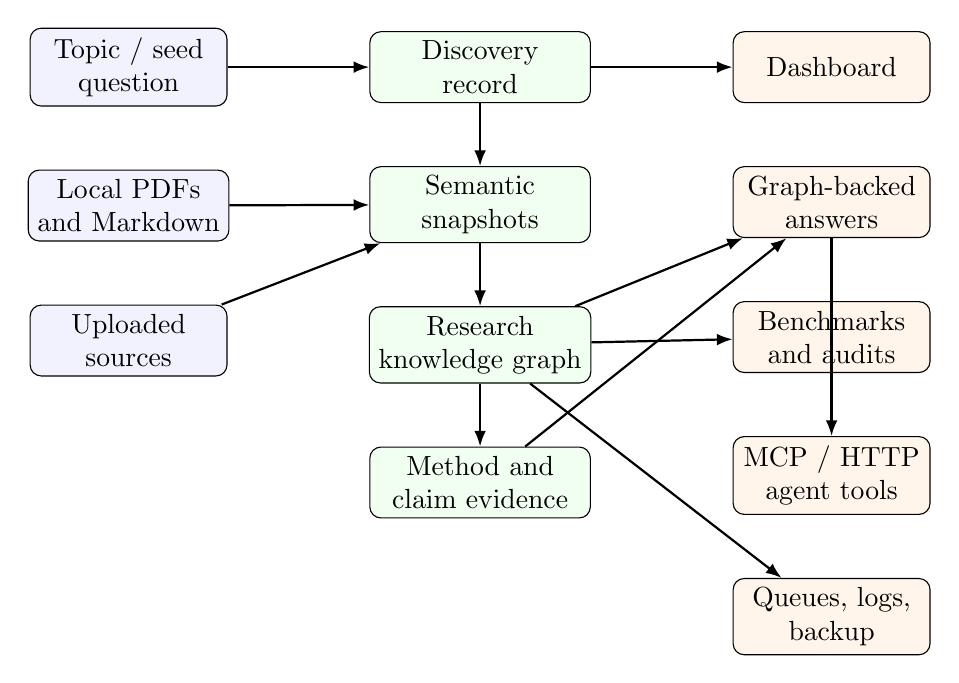
\begin{tikzpicture}[
  node distance=8mm and 9mm,
  block/.style={draw, rounded corners, align=center, minimum width=25mm, minimum height=9mm, fill=blue!5},
  mem/.style={draw, rounded corners, align=center, minimum width=28mm, minimum height=9mm, fill=green!6},
  iface/.style={draw, rounded corners, align=center, minimum width=25mm, minimum height=9mm, fill=orange!8},
  arrow/.style={-{Latex[length=2mm]}, thick}
]
  \node[block] (topic) {Topic / seed\\question};
  \node[block, below=of topic] (files) {Local PDFs\\and Markdown};
  \node[block, below=of files] (imports) {Uploaded\\sources};

  \node[mem, right=18mm of topic] (discovery) {Discovery\\record};
  \node[mem, below=of discovery] (snapshots) {Semantic\\snapshots};
  \node[mem, below=of snapshots] (graph) {Research\\knowledge graph};
  \node[mem, below=of graph] (evidence) {Method and\\claim evidence};

  \node[iface, right=18mm of discovery] (dashboard) {Dashboard};
  \node[iface, below=of dashboard] (answers) {Graph-backed\\answers};
  \node[iface, below=of answers] (eval) {Benchmarks\\and audits};
  \node[iface, below=of eval] (agents) {MCP / HTTP\\agent tools};
  \node[iface, below=of agents] (ops) {Queues, logs,\\backup};

  \draw[arrow] (topic) -- (discovery);
  \draw[arrow] (files) -- (snapshots);
  \draw[arrow] (imports) -- (snapshots);
  \draw[arrow] (discovery) -- (snapshots);
  \draw[arrow] (snapshots) -- (graph);
  \draw[arrow] (graph) -- (evidence);
  \draw[arrow] (discovery) -- (dashboard);
  \draw[arrow] (graph) -- (answers);
  \draw[arrow] (evidence) -- (answers);
  \draw[arrow] (graph) -- (eval);
  \draw[arrow] (answers) -- (agents);
  \draw[arrow] (graph) -- (ops);
\end{tikzpicture}
\caption{Functional view of \papernexus{}. Discovery, ingestion, graph memory, evidence, benchmark, agent, and operations layers are maintained as local artifacts or controlled interfaces without changing the local ownership model.}
\label{fig:functional}
\end{figure}

\subsection{Layered Responsibilities}

\begin{table}[t]
\centering
\caption{Functional layers in \papernexus{}.}
\label{tab:layers}
\begin{tabularx}{\linewidth}{@{}lY@{}}
\toprule
Layer & Role in the research workflow \\
\midrule
Discovery & Turns a topic into provider queries, merged candidates, open-access status, download manifests, and importable sources. \\
Ingestion & Converts local PDFs or Markdown into reusable paper snapshots with parser metadata and semantic extraction results. \\
Graph memory & Represents papers, problems, methods, claims, evidence, datasets, benchmarks, takeaways, ideas, and relations as a persistent local graph. \\
Evidence & Tracks method evolution, citation contexts, exact quotes, temporal direction, confidence, and blocked or ambiguous relationships. \\
Interfaces & Provides CLI, Web UI, HTTP API, local \mcp{}, remote HTTP \mcp{}, services, logs, and Python wrappers. \\
Evaluation and hygiene & Measures retrieval and task behavior, stores encrypted local secrets, and sanitizes release artifacts before publication. \\
\bottomrule
\end{tabularx}
\end{table}

The separation is practical. Discovery can be repeated without rebuilding the graph. Parsing can be retried without losing the source manifest. Graph construction can be staged and committed after inspection. Interfaces can query committed state without re-running expensive upstream work.

\section{Functional Workflows}

\subsection{Topic to Corpus}

The discovery workflow starts from a topic, seed question, related-work paragraph, venue, author, dataset, or manually supplied paper. It plans complementary queries, sends them to open metadata providers, merges candidates, expands through citations when available, and resolves legal full-text sources. It uses services such as OpenAlex~\citep{openalex}, Semantic Scholar~\citep{semanticscholar}, Crossref~\citep{crossref}, arXiv~\citep{arxivapi}, DBLP~\citep{dblp}, Europe PMC~\citep{europepmc}, CORE~\citep{coreapi}, and Unpaywall~\citep{unpaywall}.

The important output is not merely a folder of PDFs. The workflow records what was found and why a candidate could or could not enter the corpus. A result may be a resolved open PDF, a metadata-only paper, an item requiring institutional access, an access-control-blocked page, or a URL that returned HTML instead of a PDF. This distinction matters because a research assistant should not confuse ``not downloaded'' with ``not relevant'' or with ``not legally available.'' The current implementation persists discovery runs with JSON artifacts, Markdown reports, download manifests, import-task links, candidate provenance, and latest-run pointers.

\subsection{Corpus to Research Memory}

Once sources exist locally, \papernexus{} materializes them into reusable semantic snapshots. The default path parses PDF or Markdown, stores markdown cache and metadata, and allows later LLM-assisted enrichment to run as a separate stage. This gives the user a durable intermediate representation: if graph construction changes, the system can reuse prior parsing rather than starting from raw PDFs.

The staged pipeline is intentionally simple:

\begin{lstlisting}[style=pncode]
sources -> materialize -> llm-optimize -> build-graph
        -> merge-graph -> write-index
\end{lstlisting}

The key property is resumability. A user can run the full analysis once, continue after interruption, rebuild only dirty stages, or inspect stage outputs before committing a new graph.

\subsection{Research Memory to Evidence}

The graph layer makes paper-centered objects queryable. Problems, methods, claims, evidence, datasets, benchmarks, takeaways, idea fragments, and future directions become typed nodes. Relations between them become explicit edges. This enables both conventional literature exploration and higher-level reasoning tasks.

Method evolution is treated as a special evidence problem. A system should not casually claim that one method extends, improves, replaces, adapts, or uses another method. \papernexus{} therefore records method aliases, citation contexts, quote evidence, candidate relationships, accepted relationships, stubs, and diagnostics. Strong method-evolution relationships require support beyond name overlap: the relationship must be grounded in context, direction, and confidence.

\subsection{Evidence to Answers}

Research-intelligence workflows read from graph state. They can answer cross-domain questions, produce method lineages, inspect evidence for a method relationship, return a method registry, or combine these views into a unified answer. The operating invariant is that these workflows should expose existing graph evidence rather than silently generate new evidence at query time.

This gives the system a useful division of labor. Language models may help enrich snapshots or phrase responses, but the evidence substrate remains an inspectable local graph. When a researcher asks for a mechanism, lineage, or analogy, the answer can point back to the corpus state that supports it.

\subsection{Research Memory to Evaluation}

\papernexus{} now includes a retrieval-benchmark path that can evaluate the discovery and retrieval surface rather than only describe it qualitatively. The benchmark command supports closed-corpus and live-discovery modes. Closed-corpus mode follows information-retrieval semantics: the system searches a provided corpus and is scored against query relevance labels. Live mode runs the normal provider-backed discovery workflow and scores returned papers against gold identifiers or titles.

The loader surface covers custom JSON/JSONL, BEIR-style corpora and TREC qrels, LitSearch-style query/corpus exports, BioASQ question files, native TREC biomedical topics plus qrels, CSFCube faceted annotations, and flexible schemas for SAGE, ScholarQABench/OpenScholar, PaperAsk, SPARBench, and SciNetBench. The reported metrics include hit@k, exact match@k, recall@k, weighted recall@k, precision@k, F1@k, MRR@k, MAP@k, and NDCG@k. For task-style benchmarks, \papernexus{} can additionally score answer overlap, citation precision and recall, claim-label accuracy, relation/path overlap, and optional LLM-judged answer grounding.

\section{Interface Surface}

\papernexus{} exposes the same research memory through several interfaces (Table~\ref{tab:interfaces}). This is a functional choice rather than a convenience layer: different users need different levels of control over the same corpus.

\begin{table}[t]
\centering
\caption{Interface surfaces and their intended users.}
\label{tab:interfaces}
\begin{tabularx}{\linewidth}{@{}lY@{}}
\toprule
Interface & Typical use \\
\midrule
CLI & Initialize a corpus, run staged analysis, inspect status, search the graph, benchmark retrieval, manage secure environment values, export backups, and manage services. \\
Dashboard & Inspect corpus status, graph summaries, overlays, imports, runtime configuration, and human-readable views. \\
HTTP API & Integrate browser and server workflows with authenticated routes for graph, method-evidence, discovery, and research-answer queries. \\
Local \mcp{} & Give a local coding or research agent tool access over stdio. \\
Remote HTTP \mcp{} & Expose the same agent tool surface from a running server with bearer-token authentication. \\
Python wrappers & Submit imports, inspect queues, query graph state, and orchestrate remote workflows from scripts. \\
Secure environment & Keep local provider keys and runtime secrets in an encrypted file whose encryption key is held by the system keychain. \\
\bottomrule
\end{tabularx}
\end{table}

The \mcp{} surface follows the Model Context Protocol~\citep{mcp}. Its purpose is to make research memory available to agents without asking those agents to understand the internal storage layout. Important tool families include literature discovery, research lookup, research briefing, idea catalyst, and import workflow.

\section{Assurance Mechanisms}

\papernexus{} does not claim that every extracted relationship is correct. Instead, it makes uncertainty and evidence boundaries visible.

The first assurance boundary is access and parsing provenance. Discovery records whether full text is open, unavailable, restricted, blocked, or malformed, which prevents downstream tools from treating access failure as absence of evidence. Parsing and semantic extraction are separated from graph commit, so a failed parser, degenerate title, or incomplete snapshot can be detected before it pollutes the graph. This staging is deliberately conservative: it preserves imperfect intermediate artifacts as diagnostics while preventing them from being silently promoted into claims.

The second assurance boundary is graph and method-evidence validation. The graph schema constrains the kinds of objects and relationships that can be represented, while lite projections and metadata make committed state inspectable without requiring the full graph engine for every read. Strong method-evolution edges require resolved methods, citation context, quote support, confidence, temporal direction, and non-conflicting evidence. Ambiguous aliases and stubs are preserved as diagnostics rather than promoted as validated relationships, which reduces false precision in method-lineage queries.

The third assurance boundary is operational recovery and release hygiene. Queues, logs, backups, and staged commands allow the user to recover from interruptions and audit long-running work, especially when imports, PDF parsing, and LLM enrichment run over large corpora. Retrieval benchmarks separate fixed-corpus scores from live-provider scores so that provider availability, source resolution, and corpus retrieval quality remain distinct measurements. Local credentials can be loaded from encrypted secure-env storage, and public release artifacts can be sanitized so that personal account names, absolute home paths, local caches, bearer-token fixtures, and LaTeX build traces do not leak into documentation or arXiv source bundles.

\section{Functional Footprint}

Table~\ref{tab:footprint} summarizes the current feature footprint without tying the description to source files.

\begin{table}[t]
\centering
\caption{Current functional footprint.}
\label{tab:footprint}
\begin{tabularx}{\linewidth}{@{}lY@{}}
\toprule
Function & Current behavior \\
\midrule
Literature discovery & Plans queries, merges multi-provider candidates, resolves legal full text, records coverage, and bridges resolved sources into the import queue. \\
PDF and Markdown ingestion & Supports local corpora and uploaded import tasks with parser configuration, fallback parsing, markdown cache, and semantic snapshots. \\
Graph construction & Builds a typed research graph and commits a lightweight read projection for query, dashboard, and agent workflows. \\
Method evolution & Builds method registries, validates method-to-method evidence, records candidates and accepted relationships, and exposes lineage/evidence lookups. \\
Research answers & Provides graph-backed cross-domain evidence, method lineage, method evidence, method registry, and unified answer modes. \\
Retrieval evaluation & Runs fixed-corpus and live-discovery retrieval benchmarks over custom, BEIR-style, biomedical, literature-search, and graph-reasoning benchmark formats. \\
Security hygiene & Provides encrypted local secure-env storage, bearer-token authenticated server surfaces, portable path helpers, and sanitized release artifacts. \\
Operations & Supports services, logs, dashboard serving, authenticated remote \mcp{}, backup export, backup unpack, and queue inspection. \\
\bottomrule
\end{tabularx}
\end{table}

\section{Example Use Patterns}

The most direct use pattern is literature mapping. A researcher starts with a topic such as ``graph-augmented experiment planning,'' and \papernexus{} searches open metadata providers, merges duplicate candidates, records which papers have legal full-text access, imports resolved PDFs, and builds a graph that supports later search over problems, methods, claims, evidence, and datasets. The value of the workflow is not only that it finds candidate papers, but that it records the access and provenance decisions that would otherwise disappear into a download folder. That record lets the researcher distinguish a missing source from an inaccessible source, a metadata-only candidate from a parsed paper, and a graph-backed claim from an unsupported synthesis.

A second use pattern is method lineage review. A researcher asks how a method family evolved, and the system searches validated method-to-method relationships rather than relying only on name overlap or citation adjacency. It reports predecessor and successor links together with the citation contexts and quote evidence that support the relationship. This makes the difference between a substantive improvement claim and a mere background comparison visible to the user, which is essential when method lineage later informs a related-work section or a new research idea.

A third use pattern is agent-assisted research and benchmarking. A coding or research agent can connect to local or remote \mcp{} and call tools for discovery status, graph lookup, research answers, paper index lookup, import workflow, and idea-catalyst operations without scraping folders directly. The same corpus can then be evaluated through fixed-corpus or live-discovery retrieval benchmarks. In fixed-corpus mode, \papernexus{} reads a benchmark corpus, query set, and qrels, then reports ranking metrics; in live mode, the same benchmark query can exercise OpenAlex, Semantic Scholar, Crossref, arXiv, and configured optional providers. This separation makes external-provider behavior measurable without conflating it with closed-corpus retrieval quality.

\section{Evaluation and Deployment Observations}

The measured result is operational rather than competitive: the current \papernexus{} harness can run small public retrieval audits, local import stress tests, queue recovery checks, and qwen-based LLM diagnostics, but it is not yet a repeated-run benchmark result suite. The directly comparable fixed-corpus anchors show that the observed SciFact and NFCorpus rows trail published BEIR BM25 results, so the retrieval layer should be treated as an improvement target rather than as a leaderboard claim. The deployment evidence is stronger for provenance and recoverability: discovery feeds ingestion, ingestion feeds graph construction, method evidence attaches to graph memory, and intelligence workflows consume committed graph state through CLI, dashboard, HTTP, \mcp{}, and script interfaces. This section separates public benchmark audits, sub-5GB expansion measurements, external-framework comparability, and local pipeline timing so that each claim remains tied to the measurements that support it.

For the local verification run used by this report, the project passed the full Node test suite and a release-hygiene scan. The test suite passed 366 of 366 tests. The scan found no repository-text, arXiv-source, or PDF string matches for private home paths, personal account names, long bearer-token literals, OpenAI-style keys, GitHub-style tokens, or private-key blocks.

\subsection{Sub-1GB Public Benchmark Measurements}

On May 12, 2026, we ran a small public-benchmark exercise on a remote server with constrained local storage. The run was intentionally scoped to datasets below 1GB and did not write to the production Kuzu graph database. New datasets and run artifacts were placed under \code{/data1}; the existing \code{/data2} filesystem was already full. The purpose was not to claim leaderboard comparability, but to audit whether the current retrieval harness, live-provider path, and qwen-based task evaluation path can execute on small public tasks.

The remote benchmark host, recorded as jin-Super-Server at 10.126.56.41, ran Linux 6.8.0-90-generic on x86\_64. The environment audit recorded an AMD EPYC 7542 32-Core Processor, 64 logical CPUs, 125GiB RAM, Python 3.10.16 in the \code{ccd} environment, and a project-local Node \code{v22.16.0} runtime. The \papernexus{} checkout used for the run was under \code{/data1/hyq/PaperNexus}. At run time, \code{/data1} had 15T total capacity with about 3.3T available, while \code{/data2} was already full enough that new datasets, run outputs, and discovery caches were written under \code{/data1}. The qwen rows called an OpenAI-compatible \code{cliproxyapi} provider; provider-side hardware was not visible in \papernexus{} logs.

Table~\ref{tab:sub1g-benchmark-results} is therefore reported as a statistical-readiness table rather than as a formal ML comparison. Each \papernexus{} row is a single observed execution (\(n=1\)); no value is presented as a mean over repeated runs, no 95\% confidence interval is estimable, no paired significance test is valid, and no effect size is reported. The table also includes paper-reported external anchors from the most relevant benchmark papers where the task and metric can be stated precisely. These anchors are not treated as head-to-head significance tests.

\begin{table}[t]
\centering
\caption{Statistical-readiness audit for the May 12, 2026 sub-1GB benchmark exercise, with external paper-reported anchors. External values are included only where their source, task boundary, and metric can be stated; they are not repeated-run comparisons against \papernexus{}.}
\label{tab:sub1g-benchmark-results}
\tiny
\begin{tabularx}{\linewidth}{@{}l l Y Y Y@{}}
\toprule
Benchmark & \papernexus{} setting & \papernexus{} single observed value & External reported result & Comparison status \\
\midrule
SciFact & fixed; \(n=1\); 300 q / 5.2k p & nDCG@10 0.617; R@10 0.739; MRR@10 0.583 & BEIR reports nDCG@10 0.665 for BM25 and \textbf{0.688} for BM25+CE on SciFact~\citep{beir}. & Same BEIR dataset family and same nDCG@10 metric; the single \papernexus{} run is below the published BEIR BM25 and BM25+CE anchors. \\
CSFCube & fixed; \(n=1\); 50 q / 4.2k p & nDCG@10 0.162; R@10 0.016; MRR@10 0.180 & No directly matching result was found in the currently cited BEIR, LitSearch, OpenScholar, PaSa, or SPAR benchmark papers. & Diagnostic row only; keep it for faceted-retrieval regression, not for external leaderboard comparison. \\
NFCorpus & fixed; \(n=1\); 323 q / 3.6k p & nDCG@10 0.283; R@10 0.133; MRR@10 0.484 & BEIR reports nDCG@10 0.325 for BM25 and \textbf{0.350} for BM25+CE on NFCorpus~\citep{beir}. & Same BEIR dataset family and same nDCG@10 metric; the single \papernexus{} run is below the published BEIR anchors. \\
LitSearch sample100 & fixed; \(n=1\); 100 / 597 q; 64k p & nDCG@10 0.360; R@10 0.503; MRR@10 0.330 & LitSearch reports BM25 Avg. broad R@20 39.9 and specific R@5 50.0; GritLM-7B 70.8 / 74.8; GPT-4o reranking over GritLM \textbf{75.3 / 79.2}~\citep{litsearch}. & Same 64,183-paper corpus, but \papernexus{} used a 100-query sample and reports R@10/nDCG/MRR, while LitSearch reports broad R@20 and specific R@5/R@20. Directional only until official LitSearch metrics are emitted. \\
ScholarQABench live10 & live retrieval; \(n=1\); 10 / 208 q & R@10 0.300; MRR@10 0.167; 24 provider failures & OpenScholar reports answer-level ScholarQABench metrics rather than a directly matching live-provider R@10 row~\citep{openscholar}. & Diagnostic live-provider row; not directly comparable to OpenScholar because the latter uses OSDS and evaluates synthesis/citation quality. \\
ScholarQABench live10 + LLM & live + qwen; \(n=1\); 10 / 208 q & task success 0.720; answer correctness 0.720; citation F1 0.300 & On Scholar-CS, OpenScholar reports Rubric/Cite-F1 of 51.1/47.9 for OpenScholar-8B, 57.7/39.5 for OpenScholar-GPT-4o, 45.6/48.0 for PaperQA2, and 45.0/0.1 for GPT-4o without retrieval~\citep{openscholar}. & Same benchmark family but not the same setting: \papernexus{} used a 10-query live-provider sample and qwen judging, while OpenScholar uses its 45M-paper OSDS and official rubric/citation evaluation. \\
\bottomrule
\end{tabularx}
\end{table}

The fixed-corpus observations in Table~\ref{tab:sub1g-benchmark-results} support an engineering claim, not a statistical one: the benchmark harness can execute SciFact, NFCorpus, CSFCube, and a LitSearch sample~\citep{litsearch} under the tested storage constraints. Against the directly comparable BEIR nDCG@10 anchors, the observed \papernexus{} SciFact and NFCorpus rows are below published BM25 and BM25+CE results~\citep{beir}. That gap should be treated as a regression target for the retrieval harness rather than as an inferential result, because the current data contain no repeated runs and no paired per-query significance test. The LitSearch row is more realistic for literature retrieval, but the comparison is only directional until \papernexus{} reports LitSearch's official broad R@20 and specific R@5/R@20 slices. In the single LitSearch sample100 run, the 64,183-paper corpus took 23:12.54 wall-clock time and 2.27GB peak RSS. This made it a useful bottleneck diagnostic and motivated the fixed-corpus index path used for the full LitSearch run reported in Table~\ref{tab:sub5g-fixed-results}.

The live ScholarQABench observations~\citep{scholarqabench,openscholar} are likewise diagnostic rather than official. In the retrieval-only row of Table~\ref{tab:sub1g-benchmark-results}, 24 provider failures occurred across 10 queries: 21 arXiv HTTP 429 responses and 3 Semantic Scholar HTTP 429 responses. The LLM-enhanced row used the local OpenAI-compatible qwen configuration with 90-second LLM timeouts and enabled discovery request caching. It generated 10 system answers and 10 qwen judge calls with no malformed JSON in this sample. The full row still took 15:32.32 wall-clock time, or about 93.2 seconds per query, and the citation F1 of 0.300 matched the retrieval recall@10 of 0.300. The practical implication is that live-provider caching, provider backoff, query-level checkpointing, and bounded batched LLM answer/judge calls are prerequisites before these measurements can be promoted into repeated statistical experiments.

\subsection{Sub-5GB Benchmark Expansion Measurements}

The next expansion kept the same storage discipline but raised the ceiling from sub-1GB to sub-5GB public artifacts. Tables~\ref{tab:sub5g-expansion-candidates} and~\ref{tab:sub5g-metric-plan} record the task selection and metric plan that guided the run. Tables~\ref{tab:sub5g-fixed-runtime}, \ref{tab:sub5g-fixed-results}, \ref{tab:sub5g-live-diagnostics}, \ref{tab:stark-kuzu-import}, and~\ref{tab:stark-kuzu-diagnostic} report the resulting single executions. These are still statistical-readiness measurements: each row has \(n=1\), so no standard deviation, 95\% confidence interval, paired significance test, or effect size is claimed.

\begin{table}[t]
\centering
\caption{Sub-5GB benchmark expansion candidates used for the May 12, 2026 execution. The table defines task boundaries; measured values are reported in the following result tables.}
\label{tab:sub5g-expansion-candidates}
\scriptsize
\begin{tabularx}{\linewidth}{@{}l l Y Y@{}}
\toprule
Candidate & Public footprint & Comparable task & Why it belongs in the sub-5GB tier \\
\midrule
LitSearch full & About 2.85GB repository & Fixed-corpus scientific literature search over 64,183 papers and 597 queries~\citep{litsearch}. & Most direct full-scale fixed-corpus literature-search comparison. \\
BEIR TREC-COVID & About 111MB & Biomedical COVID literature retrieval with a larger corpus than SciFact/NFCorpus~\citep{beir}. & Adds large-corpus biomedical IR without leaving BEIR metrics. \\
BEIR SciDocs & About 19MB & Citation-oriented scientific-document retrieval~\citep{beir}. & Tests paper-to-paper retrieval rather than fact-verification only. \\
ScholarGym & About 861MB & Static deep-research information gathering over roughly 570k papers~\citep{scholargym}. & Strongest static alternative to unstable live-provider academic search. \\
ScholarSearch / AutoResearchBench & Query/gold artifacts are small & Live scholarly search and agentic literature-discovery diagnostics~\citep{scholarsearch,autoresearchbench}. & Measures provider behavior, resume, and multi-step search traces. \\
STaRK-MAG & Preflight required for MAG KB & Text-plus-graph retrieval over academic entities and relations~\citep{stark}. & Only useful sub-5GB candidate that stresses Kuzu graph retrieval directly. \\
\bottomrule
\end{tabularx}
\end{table}

\begin{table}[t]
\centering
\caption{Metrics and implementation work for the sub-5GB expansion candidates. This table defines what to emit before any new result can be treated as comparable.}
\label{tab:sub5g-metric-plan}
\scriptsize
\begin{tabularx}{\linewidth}{@{}l Y Y@{}}
\toprule
Target class & Primary metrics & Required implementation work \\
\midrule
LitSearch full & Official broad R@20 and specific R@5/R@20; also nDCG@10, MRR@10, latency. & Add broad/specific split reporting and persistent fixed-corpus index caching before the full 597-query run. \\
BEIR expansion & nDCG@10, Recall@50/100, MAP@10, MRR@10, index time, peak RSS. & Reuse BEIR loader; add memory guard and separate index-build time from query-evaluation time. \\
Static deep-research & Gold-paper Recall@20/50/100, paper-set F1, source coverage, trace success. & Add ScholarGym adapter, identity normalization, query checkpoints, and optional agent trace logging. \\
Live agentic search & Source Recall@20/50, Precision/F1@20/50, provider failures, retries, cache hit rate, resume success. & Add loaders for query/gold files; persist query rewrites, provider responses, cache hashes, and partial results. \\
Graph retrieval & Hit@K/Recall@K, text-only versus graph-only versus hybrid scores, relation/path evidence coverage. & Import into a bench-scratch Kuzu database, keep production graph isolated, and add graph-retrieval ablations. \\
\bottomrule
\end{tabularx}
\end{table}

The executed sequence followed this plan: TREC-COVID and SciDocs broadened fixed-corpus regression; LitSearch full ran after adding a per-run fixed-corpus index and candidate prefilter; ScholarGym tested a static deep-research corpus; ScholarSearch and AutoResearchBench were kept as live-provider diagnostics; and STaRK-MAG was isolated in a scratch Kuzu database. BioASQ, OpenScholar's OSDS, PaperSearchQA PubMed, full S2ORC, and SciNetBench remain outside this tier unless the server has a separate high-capacity scratch allocation.

\begin{table}[t]
\centering
\caption{Single-run sub-5GB fixed-corpus runtime on the 41 server. All rows used fixed-corpus mode, \code{--max-candidates 1000}, and \code{PAPERNEXUS_FIXED_CORPUS_SCAN_LIMIT=5000}. Values are not repeated-run means.}
\label{tab:sub5g-fixed-runtime}
\scriptsize
\begin{tabularx}{\linewidth}{@{}l r r r Y@{}}
\toprule
Dataset & Queries & Papers & Wall / peak RSS & Runtime note \\
\midrule
BEIR TREC-COVID~\citep{beir} & 50 & 171,332 & 8:54.15 / 2.56GB & Large qrels; useful for large-corpus latency regression. \\
BEIR SciDocs~\citep{beir} & 1,000 & 25,657 & 6:38.92 / 1.19GB & Citation-oriented paper-to-paper retrieval. \\
LitSearch full~\citep{litsearch} & 597 & 64,183 & 2:44.21 / 1.47GB & Full run after enabling the fixed-corpus index cache. \\
ScholarGym~\citep{scholargym} & 2,458 & 570,204 & 29:32.76 / 10.25GB & Required \code{NODE_OPTIONS=--max-old-space-size=16384}. \\
\bottomrule
\end{tabularx}
\end{table}

\begin{table}[t]
\centering
\caption{Single-run sub-5GB fixed-corpus retrieval metrics. Top-10 columns report nDCG@10, Recall@10, and MRR@10; top-100 columns report Hit@100, Recall@100, and nDCG@100.}
\label{tab:sub5g-fixed-results}
\scriptsize
\begin{tabular}{@{}l r r r r r r r r@{}}
\toprule
Dataset & nDCG10 & R10 & MRR10 & Hit100 & R100 & nDCG100 & Pool & Zero \\
\midrule
BEIR TREC-COVID~\citep{beir} & 0.557 & 0.014 & 0.870 & 1.000 & 0.090 & 0.381 & 0.337 & 0.000 \\
BEIR SciDocs~\citep{beir} & 0.153 & 0.157 & 0.274 & 0.763 & 0.336 & 0.214 & 0.541 & 0.073 \\
LitSearch full~\citep{litsearch} & 0.374 & 0.510 & 0.334 & 0.730 & 0.719 & 0.417 & 0.853 & 0.139 \\
ScholarGym~\citep{scholargym} & 0.142 & 0.189 & 0.147 & 0.428 & 0.330 & 0.174 & 0.466 & 0.421 \\
\bottomrule
\end{tabular}
\end{table}

The fixed-corpus rows in Tables~\ref{tab:sub5g-fixed-runtime} and~\ref{tab:sub5g-fixed-results} show that the new index path changes the operational profile. The earlier LitSearch sample100 run took 23:12.54 for 100 queries because it repeatedly scanned the corpus. The full LitSearch run completed all 597 queries in 2:44.21 after the in-memory corpus index and inverted candidate prefilter were enabled. The improvement should be treated as an engineering result, not a model-quality claim, because the scoring protocol still does not emit LitSearch's official broad R@20 and specific R@5/R@20 slices. ScholarGym is the current memory ceiling: it completed, but only after raising the Node heap to 16GB, and it still had a 0.421 zero-match rate under the 5,000-document scan limit.

\begin{table}[t]
\centering
\caption{Single-run live and agentic diagnostic results. These rows intentionally measure provider and query-shaping behavior, not closed-corpus retrieval quality.}
\label{tab:sub5g-live-diagnostics}
\footnotesize
\begin{tabularx}{\linewidth}{@{}l l l Y@{}}
\toprule
Diagnostic & Scale & Wall / latency & Observed result and failure mode \\
\midrule
AutoResearchBench sample~\citep{autoresearchbench} & 40 q; 175 gold papers & 5:24.77; 8,110.7ms/query & Hit@10 0.000; R@10 0.000; zero-match 1.000; 58 OpenAlex HTTP 400 failures and 5 Semantic Scholar HTTP 429 failures. \\
ScholarSearch diagnostic~\citep{scholarsearch} & 50 q; no usable gold papers & 4:14.39; 5,082.9ms/query & Avg. retrieved count 0.26; no retrieval metric is meaningful without gold papers; intended max-10 run evaluated 50 queries. \\
\bottomrule
\end{tabularx}
\end{table}

\begin{table}[t]
\centering
\caption{STaRK-MAG Kuzu import diagnostic. The database was built from the sub-5GB MAG artifact in a scratch run directory and did not touch the production \papernexus{} graph.}
\label{tab:stark-kuzu-import}
\footnotesize
\begin{tabularx}{\linewidth}{@{}l l l Y@{}}
\toprule
Stage & Scale & Wall / peak RSS & Main observed values \\
\midrule
CSV preparation & 1,872,968 nodes; 19,919,698 edges & 1:02.87 / 6.91GB & Wrote node and edge import files plus 84 query seed lists. \\
Kuzu COPY import & same full graph & 0:10.24 / 2.35GB & Imported all nodes and edges; scratch artifact footprint 1.4GB. \\
\bottomrule
\end{tabularx}
\end{table}

\begin{table}[t]
\centering
\caption{STaRK-MAG Kuzu retrieval diagnostic over 84 human-eval queries. Retrieval used title/name lexical seeds plus undirected 1--2 hop Kuzu expansion.}
\label{tab:stark-kuzu-diagnostic}
\footnotesize
\begin{tabular}{@{}l r r r r r l@{}}
\toprule
Method & Hit10 & Hit100 & R100 & nDCG100 & MRR & Latency \\
\midrule
Lexical-only seeds & 0.202 & 0.345 & 0.202 & 0.136 & 0.153 & included \\
Kuzu graph-expanded & 0.202 & 0.393 & 0.255 & 0.146 & 0.155 & avg 4.77s; p95 6.87s \\
\bottomrule
\end{tabular}
\end{table}

The STaRK-MAG rows in Tables~\ref{tab:stark-kuzu-import} and~\ref{tab:stark-kuzu-diagnostic} answer a different question from the fixed-corpus rows: whether Kuzu can carry a graph-retrieval diagnostic at this scale. The answer is yes for import and bounded traversal, but not yet for quality. The graph-expanded run raised Hit@100 and Recall@100, while Hit@10 stayed unchanged at 0.202. This means the current lexical seed selection and graph scoring place additional relevant papers into the candidate set but do not rank them early enough. The next graph-retrieval work should add relation-aware seed parsing, high-degree node penalties, path-type features, and a text-only versus graph-only versus hybrid ablation before claiming comparability to official STaRK results.

\subsection{Comparability to External Frameworks}

\papernexus{} is closest to academic-search and paper-centered research-agent systems, but the level of comparability depends on the task boundary. The safest presentation is to separate closed-corpus retrieval, literature-search retrieval, live academic paper search, citation-grounded QA, and method-graph evaluation. Tables~\ref{tab:beir-direct-comparison}, \ref{tab:litsearch-directional-comparison}, \ref{tab:scholarqa-directional-comparison}, \ref{tab:live-agent-comparison}, and~\ref{tab:method-graph-comparison} therefore split the comparison into task-specific views. These tables do not introduce repeated-run statistics: all \papernexus{} values remain single observed runs, and all external values are copied from the cited papers as reported anchors.

\begin{table}[t]
\centering
\caption{Direct fixed-corpus retrieval anchors on BEIR-family tasks. The gap column is a descriptive arithmetic difference between the single \papernexus{} run and the paper-reported BEIR BM25 anchor, not a significance test.}
\label{tab:beir-direct-comparison}
\scriptsize
\begin{tabularx}{\linewidth}{@{}l l l l l Y@{}}
\toprule
Dataset & Metric & \papernexus{} & BEIR BM25 & BEIR BM25+CE & Interpretation \\
\midrule
SciFact & nDCG@10 & 0.617 & 0.665 & \textbf{0.688} & Direct metric and dataset-family match; \papernexus{} is 0.048 below BEIR BM25 in this single run~\citep{beir}. \\
NFCorpus & nDCG@10 & 0.283 & 0.325 & \textbf{0.350} & Direct metric and dataset-family match; \papernexus{} is 0.042 below BEIR BM25 in this single run~\citep{beir}. \\
\bottomrule
\end{tabularx}
\end{table}

\begin{table}[t]
\centering
\caption{Directional LitSearch comparison. LitSearch reports broad-query R@20 and specific-query R@5 slices; the current \papernexus{} full run reports all 597 queries with R@10, nDCG@10, and MRR@10, so no head-to-head rank is claimed until the same broad/specific slices are emitted.}
\label{tab:litsearch-directional-comparison}
\scriptsize
\begin{tabularx}{\linewidth}{@{}l Y Y@{}}
\toprule
System or setting & Reported metrics & Comparison boundary \\
\midrule
\papernexus{} full LitSearch & R@10 0.510; nDCG@10 0.374; MRR@10 0.334; R@100 0.719 & Same 64,183-paper corpus and all 597 queries, but still different metrics from the paper's broad/specific slices. \\
LitSearch BM25 & Broad R@20 39.9; specific R@5 50.0 & Paper-reported lexical baseline~\citep{litsearch}. \\
LitSearch GritLM-7B & Broad R@20 70.8; specific R@5 74.8 & Paper-reported dense baseline~\citep{litsearch}. \\
LitSearch GPT-4o rerank over GritLM & \textbf{Broad R@20 75.3}; \textbf{specific R@5 79.2} & Direct comparison requires \papernexus{} to emit the same broad/specific slices~\citep{litsearch}. \\
\bottomrule
\end{tabularx}
\end{table}

\begin{table}[t]
\centering
\caption{Citation-grounded QA anchors. The \papernexus{} row is a 10-query live-provider diagnostic with qwen answer and judge calls; OpenScholar rows use the paper's Scholar-CS evaluation setting and are not head-to-head reproductions.}
\label{tab:scholarqa-directional-comparison}
\scriptsize
\begin{tabularx}{\linewidth}{@{}l l l l Y@{}}
\toprule
System or setting & Retrieval store & Correctness-like metric & Citation-like metric & Interpretation \\
\midrule
\papernexus{} live10 + qwen & Live OpenAlex/S2/arXiv & Answer correctness 0.720 & Citation F1 0.300 & Diagnostic only; supporting-paper R@10 was also 0.300, limiting citation quality. \\
OpenScholar-8B & OSDS 45M papers & Rubric 51.1 & Cite-F1 47.9 & Paper-reported Scholar-CS anchor~\citep{openscholar}. \\
OpenScholar-GPT-4o & OSDS 45M papers & \textbf{Rubric 57.7} & Cite-F1 39.5 & Paper-reported stronger answer-quality anchor with lower Cite-F1 than OpenScholar-8B~\citep{openscholar}. \\
PaperQA2 & Retrieval-augmented setting & Rubric 45.6 & \textbf{Cite-F1 48.0} & Paper-reported baseline in the OpenScholar comparison~\citep{openscholar}. \\
GPT-4o without retrieval & No retrieval store & Rubric 45.0 & Cite-F1 0.1 & Shows why citation-grounded tasks need retrieval rather than pure generation~\citep{openscholar}. \\
\bottomrule
\end{tabularx}
\end{table}

\begin{table}[t]
\centering
\caption{Live academic paper-search anchors. \papernexus{} has not yet run PaSa RealScholarQuery or SPARBench, so the external rows define the required future comparison rather than a current score.}
\label{tab:live-agent-comparison}
\scriptsize
\begin{tabularx}{\linewidth}{@{}l Y Y@{}}
\toprule
System or setting & Reported metrics & Required \papernexus{} counterpart \\
\midrule
\papernexus{} current live diagnostic & ScholarQABench live10: R@10 0.300; precision/F1 not reported & Not the same benchmark; only proves live-provider execution and failure logging. \\
PaSa-7B & RealScholarQuery: precision 0.5146; recall 0.6111; Recall@20 0.5798 & Run the same 50-query gold set with normalized paper identity and provider traces~\citep{pasa}. \\
SPAR & SPARBench: F1 0.3015; precision 0.2932; recall 0.3103 & Run SPARBench with the same metric definitions and cache-stamped providers~\citep{sparbench}. \\
AutoScholar & SPARBench: \textbf{F1 0.3843}; precision 0.3612; \textbf{recall 0.4105} & Treat as a stronger agentic-search anchor, not as a current \papernexus{} result~\citep{sparbench}. \\
\bottomrule
\end{tabularx}
\end{table}

\begin{table}[t]
\centering
\caption{Method-graph evaluation anchors. These are not retrieval scores; they define the kind of gold graph comparison needed before \papernexus{} can make method-evolution quality claims.}
\label{tab:method-graph-comparison}
\scriptsize
\begin{tabularx}{\linewidth}{@{}l Y Y@{}}
\toprule
System or setting & Reported graph metric & Required \papernexus{} counterpart \\
\midrule
Intern-Atlas & 30 survey-derived graphs: Node Match Ratio 91.0\%; Edge Reachable Ratio 89.7\%; Path Semantic Correctness 92.0\% & Build equivalent gold fixtures, then score canonical method matching, reachable method edges, and path semantics~\citep{internatlas}. \\
\papernexus{} current graph harness & No public method-graph score yet & Use isolated bench-scratch Kuzu databases and report text-only, graph-only, hybrid retrieval, and method-edge quality. \\
\bottomrule
\end{tabularx}
\end{table}

The strongest current claim is therefore not that \papernexus{} outperforms these systems. The defensible claim is that it now has the substrate required to compare against them in layers without erasing task boundaries. The direct BEIR comparison in Table~\ref{tab:beir-direct-comparison} identifies an immediate retrieval regression target: the observed SciFact and NFCorpus nDCG@10 values are below published BM25 anchors, while the newer TREC-COVID and SciDocs rows in Table~\ref{tab:sub5g-fixed-results} extend that regression surface. The LitSearch comparison in Table~\ref{tab:litsearch-directional-comparison} is directionally stronger after the full 597-query run, but it is still incomplete until the official broad and specific slices are emitted. The ScholarQABench comparison in Table~\ref{tab:scholarqa-directional-comparison} shows that retrieval recall and citation quality should be reported separately. The PaSa/SPAR comparison in Table~\ref{tab:live-agent-comparison} requires same-query live paper-set evaluation with provider traces, identity normalization, cache hashes, and date-stamped provider behavior. The method-graph comparison in Table~\ref{tab:method-graph-comparison} requires gold method-evolution fixtures before any claim about graph quality. AutoResearchBench, ScholarSearch, and STaRK-MAG now have diagnostic rows in this report, but they remain non-official comparisons until query rewriting, gold normalization, and official metric adapters are implemented. AstaBench, LiveDRBench, and SciNetBench remain future diagnostic targets.

\subsection{Local Pipeline Measurements}

On May 11, 2026, we ran several local measurements to separate graph commit, synchronization, PDF parsing, and LLM-based semantic enrichment latency. The tests were run against local \papernexus{} corpora and authenticated local server surfaces. Tables~\ref{tab:local-stage-timing}, \ref{tab:local-import-timing-shape}, \ref{tab:local-queue-recovery}, \ref{tab:local-llm-batch}, and~\ref{tab:local-upload-stress} report these as operational audit tables. They are not public benchmark comparisons: each condition has one independent execution unless explicitly stated, so the tables do not report between-run standard deviations, confidence intervals, exact \(p\)-values, or effect sizes. Their role is to identify bottlenecks and failure modes that must be fixed before the public benchmark rows can be turned into repeated experiments.

These operational measurements were run from the project workstation rather than the 41 benchmark host. The environment audit recorded macOS 15.1 on \code{arm64}, 10 logical CPUs, 16GB RAM, and Node \code{v25.4.0}. The upload and queue tests used authenticated local server routes; the qwen batch tests used the same local OpenAI-compatible \code{cliproxyapi} configuration, with provider-side hardware again unavailable to local logs.

\begin{table}[t]
\centering
\caption{Operational stage timing from one 10-real-paper local pipeline run. Values are within-run log summaries, not repeated-run estimates.}
\label{tab:local-stage-timing}
\scriptsize
\begin{tabularx}{\linewidth}{@{}l l l Y@{}}
\toprule
Measured stage & Unit and \(n\) & Observed timing & Statistical status and interpretation \\
\midrule
Fast graph commit & 10 papers; \(n=1\) run & 0.084 s within-run mean & No between-run std, 95\% CI, paired test, or effect size; durable writes were small in this observed workload. \\
Sync & 10 papers; \(n=1\) run & 0.59 s within-run mean & No between-run std, 95\% CI, paired test, or effect size; synchronization was not the observed bottleneck. \\
LLM optimize & 10 papers; \(n=1\) run & 113.7 s within-run mean & No between-run std, 95\% CI, paired test, or effect size; this was the dominant observed stage. \\
Active sync & 10 papers; \(n=1\) run & 120.4 s observed active window & No between-run std, 95\% CI, paired test, or effect size; the total active window tracked LLM optimization. \\
\bottomrule
\end{tabularx}
\end{table}

\begin{table}[t]
\centering
\caption{Production-style single-paper import timing audit after scoped import processing was enabled. Ranges are observed operational ranges, not confidence intervals.}
\label{tab:local-import-timing-shape}
\scriptsize
\begin{tabularx}{\linewidth}{@{}l l Y@{}}
\toprule
Stage & Observed timing & Statistical status and operational reading \\
\midrule
PDF to Markdown & 0.3--1.5 s per paper & Observed range only; no repeated-run std, 95\% CI, paired test, or effect size. \\
Materialize total & 0.4--2.2 s per paper & Observed range only; source reading, PDF conversion, Markdown cache, and snapshot creation stayed in low seconds. \\
LLM Stage 2 semantic extraction & 30--40 s per paper & Observed range only; the import task waits primarily on LLM request latency or provider throughput. \\
Fast commit & 3.5--4 s per paper & Observed range only; visible fixed latency but still smaller than LLM extraction in this path. \\
End-to-end import task & 40--46 s per paper & Observed range only; normal LLM-enhanced imports were dominated by Stage 2 in these logs. \\
\bottomrule
\end{tabularx}
\end{table}

\begin{table}[t]
\centering
\caption{Queue recovery and continue validation from one production-style import incident. Counts describe the audited incident and are not inferential statistics.}
\label{tab:local-queue-recovery}
\footnotesize
\begin{tabularx}{\linewidth}{@{}l Y Y Y@{}}
\toprule
Measurement & Before recovery & Recovery evidence & Final active queue state \\
\midrule
Historical queue audit & 117 completed tasks and 33 failed tasks. & All 33 uploaded source files still existed; 24 were PDF uploads and 9 were Markdown uploads; all 33 had equivalent completed imports later in the queue. & 117 completed, 0 failed, 0 pending, 0 running, and overall progress at 100\%. \\
\bottomrule
\end{tabularx}
\end{table}

\begin{table}[t]
\centering
\caption{Single-prompt multi-paper LLM extraction audit using local \code{cliproxyapi} with \code{qwen3.6-plus} and thinking disabled. Each condition was executed once.}
\label{tab:local-llm-batch}
\scriptsize
\begin{tabularx}{\linewidth}{@{}r l Y Y@{}}
\toprule
Papers in one prompt & Observed completion time & Result & Statistical status and interpretation \\
\midrule
1 & 4.992 s & HTTP 200 with parseable structured output. & \(n=1\); no std, 95\% CI, paired test, or effect size; establishes only a one-paper smoke trace. \\
10 & 45.561 s & HTTP 200 with parseable structured output. & \(n=1\); no std, 95\% CI, paired test, or effect size; small multi-paper batching is feasible in this observed trace. \\
100 & 256.409 s & HTTP 200, but the response was truncated at 60,848 characters and JSON parsing failed. & \(n=1\); no std, 95\% CI, paired test, or effect size; a 100-paper single prompt is not production-safe. \\
\bottomrule
\end{tabularx}
\end{table}

\begin{table}[t]
\centering
\caption{Authenticated PDF upload and import stress audit. Each condition used one fresh temporary corpus with one seed Markdown source, so committed paper counts are one larger than the number of uploaded PDFs.}
\label{tab:local-upload-stress}
\scriptsize
\begin{tabularx}{\linewidth}{@{}r l l l l Y@{}}
\toprule
Uploaded PDFs & Request payload & Enqueue latency & End-to-end time & Materialize / PDF parse & Statistical status and committed graph \\
\midrule
1 & 182,972 bytes & 14 ms & 2.026 s & 1.443 s / 1.417 s & \(n=1\); no std, 95\% CI, paired test, or effect size; 2 papers, 25 nodes, 55 edges. \\
100 & 18,292,646 bytes & 60 ms & 30.289 s & 113.589 s / 110.907 s & \(n=1\); no std, 95\% CI, paired test, or effect size; 101 papers, 223 nodes, 1,837 edges. \\
\bottomrule
\end{tabularx}
\end{table}

The upload stress audit in Table~\ref{tab:local-upload-stress} used the HTTP import route with base64 file payloads, the background import worker, the MarkItDown PDF parser, four-way analysis concurrency, and \code{semanticExtraction=heuristic-only}. Therefore the measured path includes upload, queueing, PDF-to-Markdown conversion, materialization, the pipeline's LLM-optimization stage in heuristic-only mode, and fast graph commit, but excludes external LLM enrichment calls. The 100-PDF condition completed without failed import tasks in its single run. Its additional cumulative substage timings were 0.418 seconds for Markdown reads, 0.499 seconds for Markdown parsing, and 1.665 seconds for semantic snapshots. Because parsing ran concurrently, 113.589 seconds of cumulative materialization work completed in 30.289 seconds of wall time, or roughly 3.3 uploaded PDFs per second for this small-PDF workload. This throughput is a practical observation, not a statistically significant estimate.

Taken together, these audit tables support cautious engineering conclusions. The current graph write and synchronization path was not the observed bottleneck in the tested runs. Without external LLM enrichment, PDF-to-Markdown conversion dominated the import path. With LLM enrichment enabled, the LLM-optimization stage dominated graph commit in both the single-import timing logs and the aggregate 10-paper pipeline log. The queue-recovery audit also validates the intended continue behavior: stale historical failures can be reconciled without deleting task logs or uploaded sources, while the active queue presents the recovered state to agents. The CPA/Qwen batch audit shows why the system should not optimize by sending arbitrarily large paper batches to a single prompt: the 10-paper condition worked once, while the 100-paper condition returned HTTP 200 with unusable truncated JSON. The safer production design is prompt-budget batching, deterministic schema validation, batch-level checkpoints, and split retry/continue for malformed or oversized outputs.

This conclusion is consistent with the staged extraction design studied from Intern-Atlas~\citep{internatlas}. That system does not rely on one giant prompt over full papers. It parses PDFs into structured sections using Nougat for born-digital PDFs and GROBID as a fallback, then runs a two-phase LLM extraction process over selected evidence. The first phase uses Introduction and Method sections plus reference titles and abstracts, averaging about 21.2 references and 5.8k input / 2.1k output tokens per prompt. The second phase only processes non-background candidates, batches about 10 candidates at a time, averages about 7.9k input / 2.8k output tokens, and repairs malformed batches once before dropping persistent failures. For \papernexus{}, the practical implication is to keep full-text parsing local and reusable, feed the LLM only the sections needed for the target extraction, and make every LLM batch independently resumable.

\section{Limitations and Future Work}

\papernexus{} has several current limitations that matter for interpreting the reported measurements. Metadata-only discovery candidates are recorded but are not automatically promoted into full graph paper nodes unless they pass through import and materialization. Discovery source coverage remains incomplete: OpenReview, Papers with Code, DataCite, OpenAIRE, BASE, HAL, Zenodo, bioRxiv, medRxiv, SSRN, OSF, and Chinese scholarship providers are natural extensions. Systematic-review-style screening is not yet a standalone workflow with include/exclude tables and reviewer decisions, and version relations such as preprint-of, extended-by, artifact-for, and dataset-for are not yet fully represented as graph relations. Method-evolution quality also depends on extraction quality; conservative validation reduces false positives but may miss valid relationships that are weakly expressed in source text.

The evaluation limitations are equally important. The benchmark layer has loaders and metrics, but the current public numbers are single executions rather than repeated experiments. The sub-1GB and sub-5GB runs show that the harness can execute fixed-corpus retrieval, live retrieval, qwen-based task evaluation, static deep-research retrieval, and scratch Kuzu graph diagnostics under the tested storage constraints, but they do not establish statistical significance or leaderboard-level superiority. Future evaluation should therefore focus on discovery recall against systematic-review gold sets, open-access status accuracy, parser success and metadata accuracy, graph entity and relation precision, method-edge precision, fixed-corpus retrieval quality, live-provider retrieval quality, answer faithfulness, and official metric adapters for LitSearch, ScholarGym, STaRK-MAG, ScholarSearch, and AutoResearchBench. These measurements should be paired with engineering checks for latency, throughput, queue recovery, service stability, and secure release hygiene.

\section{Conclusion}

\papernexus{} is a local-first research harness for turning paper-centered work into durable, inspectable research memory. Its main contribution is not a single retrieval model or a single agent prompt, but the integration of discovery, ingestion, graph construction, method-evidence validation, graph-backed research intelligence, benchmark execution, and multi-surface operation into one local workflow. The current evidence supports a constrained but useful conclusion: the system can preserve provenance across sources, snapshots, graph state, agent interfaces, queue recovery, and preliminary benchmark audits, while its retrieval quality and LLM-enriched paths still require repeated evaluation and targeted optimization. \papernexus{} is therefore best understood as research infrastructure for automation with provenance, where generation is downstream of memory, evidence, and measurement.

\section*{Acknowledgments}

This report was generated from the local \papernexus{} working tree and project documentation on May 12, 2026. The writing style was revised to follow the functional technical-report pattern exemplified by ARIS~\citep{yang2026aris}; no text from that paper is reused.

\bibliographystyle{plainnat}
\bibliography{references}

\appendix

\section{Functional Command Sketch}

The most common operator path is:

\begin{lstlisting}[style=pncode]
papernexus init
papernexus analyze --force
papernexus serve
\end{lstlisting}

The staged path exposes intermediate state:

\begin{lstlisting}[style=pncode]
papernexus materialize --continue
papernexus llm-optimize --continue
papernexus build-graph --continue
papernexus merge-graph --continue
papernexus write-index --continue
\end{lstlisting}

Retrieval evaluation can be run in fixed-corpus mode:

\begin{lstlisting}[style=pncode]
papernexus benchmark-retrieval ./benchmarks/scifact \
  --format beir \
  --evaluation-mode fixed-corpus \
  --k 1,5,10,20
\end{lstlisting}

Local secrets can be stored outside plain configuration files:

\begin{lstlisting}[style=pncode]
papernexus secure-env set OPENAI_API_KEY
papernexus secure-env list
\end{lstlisting}

\section{Remote Agent Pattern}

Remote agent access is enabled by running the dashboard server with authenticated streamable HTTP \mcp{}. A client can then call graph lookup, literature discovery, import workflow, and idea-catalyst tools against the same corpus that the local dashboard displays. This pattern is useful when the research corpus stays on one machine but agents or scripts run from another environment.

\end{document}
